%*****************************************
\chapter{Realisierung}\label{ch:Realisierung}
%*****************************************
    Bei der Realisierung eines anomaliebasierten \ac{IDS} müssen, wie in~\autoref{ch:Grundlagen} beschrieben, zwei Phasen durchlaufen werden.
    Die Trainingsphase und die Testphase.
    Diesen beiden Phasen muss ein präparierter Datensatz und die Definition der exakten Eingaben und Ausgaben des \acp{LSTM} zu Grunde liegen. 
    Welche Datensätze überhaupt in Frage kommen, wurde bereits in~\autoref{sec:Datensatz} untersucht.
    In~\autoref{sec:Tools} werden verschiedene Tools und Ressourcen betrachtet, die für die Vorverarbeitung des Datensatzes und weitere Implementierungen nötig sind.
    Wie dieser für das \ac{LSTM} vorbereitet wird, und welche Informationen neben dem Namen des System Calls verwendet werden, wird in~\autoref{sec:Preprocessing} betrachtet. %KOMMA
    Der eigentliche Algorithmus, also das Finden von Anomalien in den Daten, wird in~\autoref{sec:Algorithmus} beschrieben.
    Dabei wird erst eine allgemeine Beschreibung des Ablaufes gegeben und anschließend detailliert auf Training und Anomalieerkennung eingegangen.
    In \autoref{sec:parameterwahl} werden die festgelegten Parameter und die Parameter, welche in den Experimenten untersucht werden, vorgestellt.
    Dieses Kapitel wird dann in~\autoref{sec:Metriken} mit einer Untersuchung der Metriken abgeschlossen, die für die Auswertung der Experimente benötigt werden. 

    \section{Verwendete Bibliotheken und Ressourcen}\label{sec:Tools}
        Für die Implementierung der folgenden beschriebenen Verfahren kommen verschiedene Bibliotheken zum Einsatz.
        Die gesamte Implementierung wurde in Python $3.7$ umgesetzt.
        Um das \ac{W2V}-Verfahren einzubinden, wird die \ac{W2V} Implementierung der GENSIM Bibliothek~\cite{GENSIM} genutzt.
        Für die Implementierung des \acp{LSTM} wird die PyTorch Bibliothek~\cite{PYTORCH} angewandt. 
        Berechnungen für diese Arbeit wurden (z.T.) mit Ressourcen des Universitätsrechenzentrums Leipzig durchgeführt.

    \section{Vorverarbeitung}\label{sec:Preprocessing}
        %In dem kommenden Abschnitt~\ref{sec:struktur} wird die erste Vorverarbeitung des Datensatzes vorgestellt.
        Im kommenden~\autoref{sec:syscalldarstellung} soll untersucht werden, welche Darstellungsformen für System Calls im Rahmen dieser Arbeit interessant und sinnvoll sind.
        Dabei werden die System Call Daten praxisnah als Datenstream betrachtet.
        Weshalb in~\autoref{sec:streamdarstellung} die Frage geprüft wird, wie dieser für das \ac{LSTM} dargestellt wird.
        Ein weiterer wichtiger Teil der Arbeit besteht darin zu klären, welche Metadaten neben dem Namen des System Calls noch verwendet werden können, um die Erkennungsrate der Angriffe zu erhöhen, bzw.\ die Fehlerrate zu verringern.
        Die Frage, welche Informationen dafür verwendet werden können und wie diese dargestellt werden, wird in~\autoref{sec:Meta} behandelt.

        \subsection{Darstellung eines System Calls}\label{sec:syscalldarstellung}
            Neuronale Netze benötigen numerische Werte, weswegen eine Umwandlung der Namen der System Calls stattfinden muss, sodass die Sequenz dem neuronalen Netz als Eingabe dienen kann. 
            Eine einfache Kodierung dieser Strings bestünde darin, die System Calls in Integer Werte umzuwandeln.
            Allerdings entstehen dabei künstliche Zusammenhänge und Ordnungen, welche für den Lernvorgang unvorteilhaft sein können~\cite{NEURALBISHOP1995}.
            Doch es bieten sich verschiedene Alternativen, um diese künstlichen Zusammenhänge zu verhindern.
            Zwei mögliche Verfahren werden im Folgenden behandelt.

            \paragraph{One-Hot-Encoding}
                Für die Darstellung eines System Calls mit dem \ac{OHE} muss zunächst die Anzahl $k$ der unterschiedlichen System Calls ermittelt werden.
                Der System Call $sc_i$ aus der Menge der möglichen System Calls $ SC = \{sc_1,sc_2,\dots,sc_k\}$ wird dann als Bit-Vektor $v_i$ der Länge $k$ kodiert.
                Dabei nehmen alle Stellen bis auf $i$ den Wert $0$ an und sonst den Wert $1$.
                So wird aus dem System Call \textit{open} aus der Menge $SC = \{open, close, read\}$ der Vektor $v_1 = (1, 0, 0)$.
                Und für \textit{close} gilt dann $v_2 = (0,1,0)$.
                Da die Anzahl der möglichen System Calls, also $k$ begrenzt ist, scheint diese Darstellung für einen System Call denkbar.
                Allerdings bringt sie auch zwei neue Probleme mit sich.
                Zum einen führt das \ac{OHE} eines System Calls bei großem $k$ zu einem langen und spärlich besetzten Vektor $v_i$.
                Gerade bei neuronalen Netzen führt das zu längeren Rechenzeiten.
                Und der neu gewonnen Vorteil, dass keine künstlichen Ordnungen vorhanden sind birgt den Nachteil, dass ebenso tatsächlich vorhandene Zusammenhänge verloren gehen.
                So besteht ein Zusammenhang zwischen \textit{open} und \textit{close}, da zum Beispiel Dateien, welche geöffnet werden, in der Regel auch wieder geschlossen werden müssen.
                Dieser Zusammenhang ist in dem \ac{OHE} verloren gegangen. 
                Optimaler Weise gilt es also eine Darstellung zu finden, die kurz ist und in welcher nur gewollte Ordnungen vorhanden sind.
            \paragraph{Word2Vec}
                In der \ac{NLP} gilt es ähnliche Probleme durch die Darstellungen der Wörter zu lösen.
                Das \ac{W2V} Verfahren ist ein auf feedforward neuronalen Netzen basierender Ansatz, welcher in der \ac{NLP} häufig eingesetzt wird~\cite{W2VAYYADEVARA2018}.
                Dabei werden Wörter aus einem gegebenen Satz an möglichen Wörtern anhand eines Trainingsdatensatzes in dichte Vektoren $v_{w2v}$ fester Länge $e$ kodiert beziehungsweise \textit{embedded}\marginpar{zu dt.\ eingebettet}.
                Also ein System Call $sc_i$ aus der Menge $SC = \{sc_1,sc_2,\dots,sc_k\}$ wird umgewandelt in einen Vektor $v_{w2v}$ mit gegebener Länge $e$.
                Ziel des von~\cite{W2VMIKOLOV2013} eingeführten \ac{W2V} Verfahrens ist es, eine Dimensionsreduktion durchzuführen, bei welcher möglichst viel Kontextinformationen erhalten bleiben.
                So sollen also die Vektordarstellungen von ähnlichen Wörtern ebenso ähnlich sein.
                Ähnlich meint in diesem Zusammenhang eine semantische Ähnlichkeit.
                Ziel ist es also, dass die Vektordarstellungen von zwei schreibenden System Calls näher beieinander liegen, als die Darstellung eines schreibenden System Calls und einem System Call zur Prozesskontrolle. 
                Dies wird erreicht, indem Worte für das Erstellen der Kodierung nicht einzeln betrachtet werden, sondern immer in einem Kontext.
                Es wird angenommen, dass Wörter die häufig in einem ähnlichen Kontext auftreten, auch ähnlich sind.
                Dabei sind mit Kontext die Wörter vor und nach dem aktuellen Wort gemeint.
                Wie umfangreich dieser Kontext für jedes Wort sein soll, wird mit der Fenstergröße $w$ festgelegt.
                In der Trainingsphase gibt es zwei verschiedene Architekturen.
                \textit{Continuous Bag-Of-Words} versucht das feedforward Netzwerk darauf zu trainieren eine Vorhersage über ein Wort anhand des Kontextes zu machen.
                Hingegen wird unter Verwendung von \textit{Skip-gram} eine Vorhersage des Kontextes aufgrund des Wortes trainiert.~\cite{EMBEDDINGPILEHVAR2020}
                Schwierigkeiten wie das häufige Auftreten von Wörtern in der englischen Sprache wie \textit{the}, treten in der System Call Domäne nicht auf.
                Auch Grimmer et al.~\cite{IDSTHREADGRIMMER2021} nutzen bereits die Vorteile der dicht besetzten und dimensionsreduzierten Vektoren in anomaliebasierten \ac{HIDS} mit System Calls.

            In~\cite{W2VWUNDERLICH2019} wird beschrieben, dass das \ac{OHE} laut Ergebnissen bevorzugt werden sollte, wobei auch das \ac{W2V} geeignet ist.
            In dieser Arbeit überwiegt allerdings der zeitliche Vorteil\marginpar{mehr dazu in \autoref{sec:erg_time}} durch die Dimensionsreduktion des \ac{W2V}.
            Neben den eigentlichen Namen des System Calls, enthalten tatsächliche System Calls wie in \autoref{sec:syscalls} beschrieben noch wesentlich mehr Informationen.
            Wie zumindest Teile dieser die Embeddings der System Calls erweitern können, soll im folgenden Abschnitt untersucht werden.

        \subsection{Darstellung weiterer Parameter}\label{sec:Meta}
                Wie zusätzliche Informationen der System Calls genutzt werden können ist auch Gegenstand bestehender Forschung.
                In \autoref{sec:related_sys_arg} wurden die verschiedenen bestehenden Ansätze untersucht.

                Im Folgenden soll es speziell darum gehen, neue Darstellungsformen der System Call Argumente zu finden.
                Dabei soll noch einmal kurz auf die in \autoref{sec:syscalls} besprochenen Grundlagen zurückgegriffen werden, um einen ersten Anhaltspunkt für wichtige Informationsquellen zu finden.

                Um die Unterscheidung von Normalverhalten und einer Anomalie zu erleichtern, müssen Faktoren betrachtet werden, welche sensibel auf eine Veränderung des Normalverhaltens reagieren.
                Gleichzeitig sollen dabei aber nicht einzelne Angriffe genutzt werden um diese Faktoren zu ermitteln.
                Denn dabei besteht die Gefahr, Signaturen einzelner Angriffe abbilden zu wollen, was wie in \autoref{sec:Datenanalyse} ungewollte Nachteile hat.
                Ziel dieses Abschnitts ist es, die Überlegungen und Umsetzungen von zwei Verfahren zur Darstellung von zusätzlichen System Call Informationen zu präsentieren.

                \paragraph{Zeitliche Abstände von System Calls}
                    Wie bereits in \autoref{sec:related_sys_arg} beschrieben, verwenden Lucket et al.~\cite{TIMINGLUCKETT2016} die Timing-Information von System Calls für das Aufspüren von Rootkits.
                    In diesem Abschnitt wird diese Idee wieder aufgegriffen.
                    Die Grundidee besteht darin, dass durch ein Angriffsverhalten eine zumindest kurzzeitige Veränderung im Timing der auftretenden System Calls eintritt.
                    Dabei gelten System Calls in diesem Ansatz nur als aufeinanderfolgend, sofern sie auch aus dem selben Thread stammen.
                    Eine genauere Erläuterung dazu erfolgt in \autoref{sec:streamdarstellung}.
                    Um den Unterschied in den Normaldaten und Angriffsdaten zu untersuchen, wurden in \autoref{fig:time_delta} die Häufigkeit zeitlicher Abstände zwischen aufeinanderfolgenden System Calls aus dem Bruteforce und dem CVE-2019-5418 Szenario des \ac{LID-DS} geplottet.
                    In Blau sind die Abstände der System Calls während des Normalverhaltens eingetragen und in Rot die des Normalverhaltens mit zusätzlichen Angriffsverhalten.
                    Im rechten Plot ist kein sichtlicher Unterschied zwischen Angriffsverhalten und dem Normalverhalten zu erkennen.
                    Der in diesem Szenario durchgeführte Angriff scheint nicht zu einer Abweichung der Zeitabstände zwischen System Calls zu führen.
                    Im linken Plot hingegen ist eine Abweichung im Bereich ab ca. $0.05*10^{6}$\textit{ns} zu erkennen.

                    %Wie in \autoref{sec:related_no_arg} beschrieben können Verfahren die keine weiteren Parameter verwenden umgangen werden, indem weitere System Calls eingefügt werden~\cite{Syscallseqexploit1}.
                    \begin{figure}
                        \centering
                        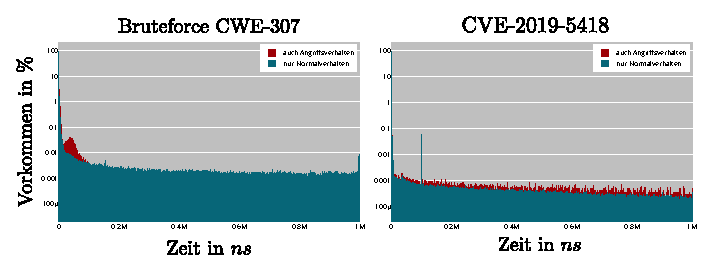
\includegraphics[width=\textwidth]{images/CVE-2012--Test-data-time_delta.eps}
                        \caption[Zeitliche Abstände zwischen System Calls]{Dargestellt ist der zeitliche Abstand zwischen zwei System Calls aus dem selben Thread.
                                 Diese werden in ihrer Häufigkeit in Prozent an allen auftretenden Abstände in dem Plot eingetragen.
                                 Verwendet wurden dafür nur die Testdaten. Links für das Bruteforce Szenario und rechts für das CVE-2019-5418 Szenario.
                                 Blau: Nur Normalverhalten, Rot: Normalverhalten und Angriffsverhalten}
                        \label{fig:time_delta}
                    \end{figure}

                    Die Umsetzung der beschriebenen Idee wird erreicht, indem der zeitlichen Abstand $\tau$ zwischen zwei aufeinanderfolgenden System Calls berechnet wird.
                    Dieser wird normalisiert als weiterer Eingabeparameter für den verarbeitenden Algorithmus verwendet.
                    In der Trainingsphase wird zunächst nur der größte Abstand $\tau_{max}$ aus den Trainingsdaten ermittelt.
                    Mithilfe dieses Wertes werden dann in der Testphase alle Werte, wie in \autoref{eq:time_norm} beschrieben, normalisiert.
                    \begin{equation}\label{eq:time_norm}
                        \tau_{norm} = \frac{\tau}{\tau_{max}}
                    \end{equation}
                    So gilt für die meisten Werte $\tau_{norm}=[0;1]$.
                    Falls $\tau\geq\tau_{max}$ gilt, kann dieser Wert auch größer als $1$ werden.

                    Doch treten mit der Verwendung dieser Information als Extraparameter zwei Probleme auf.
                    Zum einen stellt sich die Frage, ob eine Verbesserung eines Szenarios mit abweichenden Abständen\marginpar{zw. Normal- und Angriffsverhalten} eine Verschlechterung in Szenarien, in welchen dies nicht der Fall ist, zur Folge hat.
                    Und zum anderen stellt sich die generelle Frage, ob diese Information den möglichen Ergebnisraum wesentlich vergrößert, worunter die Ergebnisqualität im Gesamten leidet.
                    Denn das Betriebssystem selbst beeinflusst die Timings der System Calls.
                    So können Informationen eingebettet werden, welche wenig Aussagekraft über das Normalverhalten eines Prozesses haben.
                    Ob dies das Lernen des Normalverhaltens verbessert oder verschlechtert, wird in \autoref{sec:erg_LSTM_extra} untersucht.
                    %\begin{figure}
                        %\centering
                        %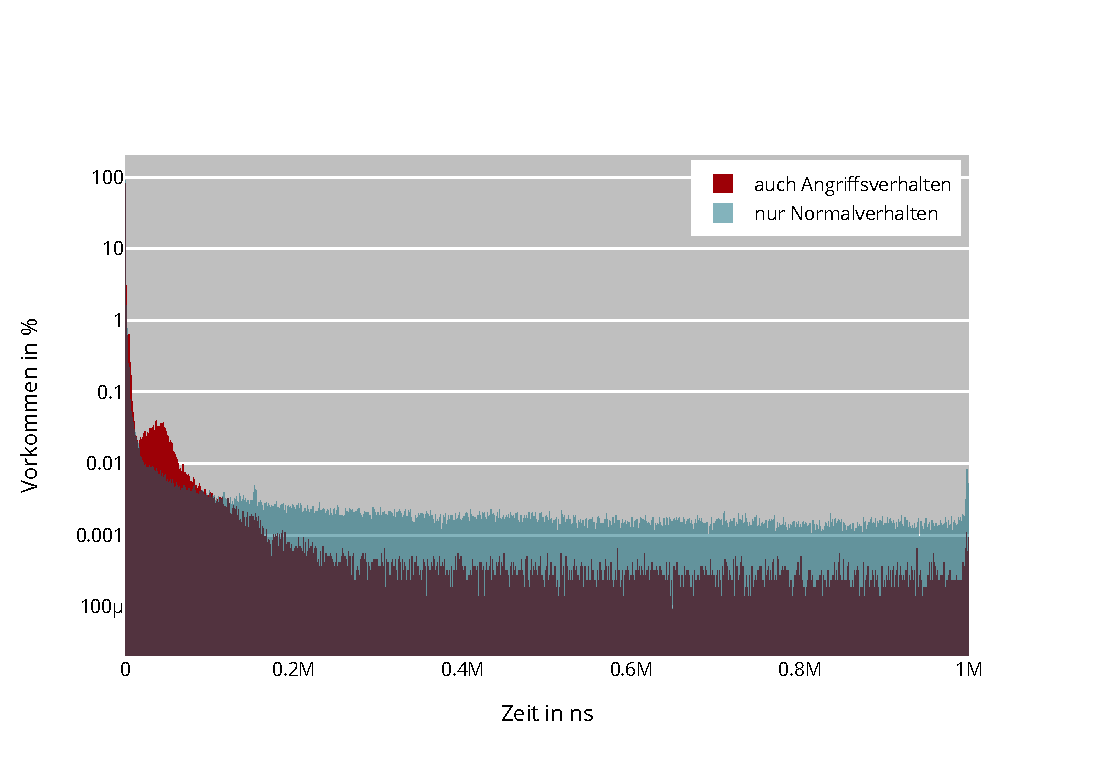
\includegraphics[width=\textwidth]{images/CVE-2012--Test-data-time_delta.pdf}
                        %\caption{Dargestellt ist der zeitliche Abstand zwischen zwei System Calls aus dem selben Thread.
                                 %Diese werden in ihrer Häufigkeit in Prozent an allen auftretenden Abstände in dem Plot eingetragen.
                                 %Verwendet wurden dafür nur die Testdaten des 
                                 %Blau: Nur Normalverhalten}
                        %\label{fig:time_delta_werte}
                    %\end{figure}

                \paragraph{Return Werte}

                    Wie in \autoref{sec:syscall_allg} angemerkt, besteht ein System Call aus zwei \glqq Phasen\grqq.
                    Wobei die zweite Phase den Rückgabewert des Betriebssystemskernels, beinhaltet.
                    Bei erfolgreicher Durchführung besteht dieser Rückgabewert bei verschiedenen System Calls aus einem positiven Integerwert.
                    Ist die Durchführung jedoch nicht erfolgreich, wird ein Fehler zurückgegeben.
                    Dieser besteht aus einem negativen Integerwert und in manchen Fällen noch einem zusätzlichem Fehlercode.
                    So gibt der Rückgabewert eines \textit{write} System Calls an, wieviele Bytes gelesen wurden.
                    Auch weitere schreibende und lesende System Calls geben die gelesenen oder geschriebene Bytes zurück.
                    Für manche System Calls, die im Zusammenhang mit Sockets stehen, gilt dies ebenfalls.
                    Der Rückgabewert enthält in diesen Beispielen also Informationen über den tatsächlichen Ablauf des spezifischen System Calls.
                    Im Folgenden wird beschrieben, wie diese Zusatzinformation der Rückgabewerte kodiert werden kann.
                    Dabei werden nur System Calls betrachtet, welche Daten schreiben oder lesen und Daten über Sockets empfangen oder senden. 
                    Zusätzlich wird dies nur für System Calls, welche auch im Datensatz vorkommen und einen Byte Rückgabewert haben, untersucht.
                    Leider fallen dabei System Calls wie \textit{send} heraus, da der Rückgabewert die Anzahl der gesendeten Charaktere angibt und nicht die Anzahl an geschriebenen Bytes.
                    Es kann also nicht davon ausgegangen werden, dass jegliche schreibende oder lesende Aktion damit abgedeckt ist.
                    In \autoref{tab:syscall_return} werden die den Anforderungen entsprechenden System Calls mit einer Kurzbeschreibung vorgestellt.

                    \begin{table}[ht]
                        \small
                        \centering
                        \begin{tabular}{cp{6cm}p{3cm}}
                            \hline
                            \rowcolor{GruvGray!36}
                            \multicolumn{3}{c}{System Calls}\\
                            \hline
                            Name & Beschreibung & Rückgabewerte\\
                            \hline
                            \hline
                            \rowcolor{GruvGray!16}
                            %open& Öffnet die von \textit{pathname} spezifizierte File. Falls diese nicht existiert kann sie mit dem Zusatz \textit{O_CREAT} automatisch erstellt werden & path, asdklfjs, slddk\\
                            write   & Schreibt angegebene Anzahl an Bytes aus dem Buffer in die Datei, welche über den Filedeskriptor $fd$ definiert wird. & Geschriebene Bytes oder $-1$ bei Fehler\\
                            pwrite  & Schreibt angegebene Anzahl an Bytes aus dem Buffer in die Datei, welche über den Filedeskriptor $fd$ definiert wird. Dabei wird der Datei-Offset nicht geändert.& Geschriebene Bytes oder $-1$ bei Fehler\\
                            \rowcolor{GruvGray!16}
                            writev  & Schreibt \textit{iovcnt} Vektor in die Datei, welche über den Filedeskriptor $fd$ definiert wird.& Geschriebene Bytes oder $-1$ bei Fehler\\

                            read    & Versucht angegebene Anzahl an Bytes von Filedeskriptor \textit{fd} zu lesen und passt den Datei-Offset an.                                              & Gelesene Bytes oder $-1$ bei Fehler\\
                            \rowcolor{GruvGray!16}
                            pread   & Versucht angegebene Anzahl an Bytes von Filedeskriptor \textit{fd} zu lesen und passt den Datei-Offset nicht an.                                        & Gelesene Bytes oder $-1$ bei Fehler\\
                            readv   & Liest spezifizierten \textit{iovcnt} Vektor aus Filedeskriptor \textit{fd} & Gelesene Bytes oder $-1$ Fehler\\

                            \rowcolor{GruvGray!16}

                            sendfile & Kopiert Daten zwischen zwei Filedeskriptoren. Kopiervorgang findet im Kernel statt.& Geschriebene Bytes oder $-1$ bei Fehler\\
                            sendmsg & Übermitteln einer Nachricht an einen anderen Socket. & Gesendete Bytes oder $-1$ bei Fehler\\
                            \rowcolor{GruvGray!16}
                            recv & Empfängt Daten von einem Socket. & Empfangene Bytes oder $-1$ bei Fehler\\
                            \makecell{recvfrom, recvmsg}& Empfängt Daten auf einem Socket welcher nicht zwingend verbindungsorientiert sein muss. & Empfangene Bytes oder $-1$ bei Fehler\\
                            \hline
                        \end{tabular}
                        \caption[Kurzbeschreibung System Calls]{Kurzbeschreibung ausgewählter System Calls.~\cite{SYSCALL_MANPAGE}}
                        \label{tab:syscall_return}
                    \end{table}
                    Diese werden in ihrer Häufigkeit in Prozent an allen auftretenden Rückgabewertgrößen in dem Plot eingetragen. 
                    Für die beschriebenen System Calls werden in \autoref{fig:return_values} die normalisierten Byte Rückgabewerte dargestellt.                
                    Beispielhaft wird dafür das $CVE-2017-7529$ Szenario genutzt.
                    Für die System Calls read, pread und readv sind die Rückgabewertgrößen im Normalverhalten wie im Normalverhalten mit zusätzlichem Angriffsverhalten gleich und zwar ca.\ $615$ Bytes.
                    Bei allen anderen betrachteten Rückgabewerten ist ein Unterschied in den auftretenden Größen bei zusätzlichem Angriffsverhalten zu erkennen.
                    So zum Beispiel bei den write, pwrite, und writev System Calls.
                    Im Normalverhalten werden entweder $100$ oder ca. $250$ Bytes geschrieben, im Angriffsverhalten kommen noch weitere sehr selten auftretende Größen vor.
                    Auch hier gilt analog zu den Zeitabständen für die Normalisierung $\rho_{norm}$ mit einem Rückgabewert $\rho$ und dem Maximalwert aus den Trainingsdaten $\rho_{max}$ aus den Trainingsdaten:
                    \begin{equation}\label{eq:return_norm}
                        \rho_{norm} = \frac{\rho}{\rho_{max}}
                    \end{equation}
                    Neben dem normalisierten Rückgabewert kann aber auch ein Fehlerwert Details über den Ablauf eines System Calls liefern.
                    Wie in \autoref{tab:syscall_return} beschrieben, wird bei diesen System Calls bei nicht erfolgreicher Durchführung eine $-1$ zurückgegeben.
                    Weshalb $\rho_{norm} = -1$ gilt, falls ein System Call aus \autoref{tab:syscall_return} einen Fehlerwert liefert.
                    %TODO noch mehr schreiben?
                    Wie sich die Verwendung der normalisierten Rückgabewerte spezieller System Calls auf die Ergebnisse auswirkt, wird in \autoref{sec:erg_LSTM_extra} behandelt.
                    
                    \begin{figure}[ht]
                        \centering
                        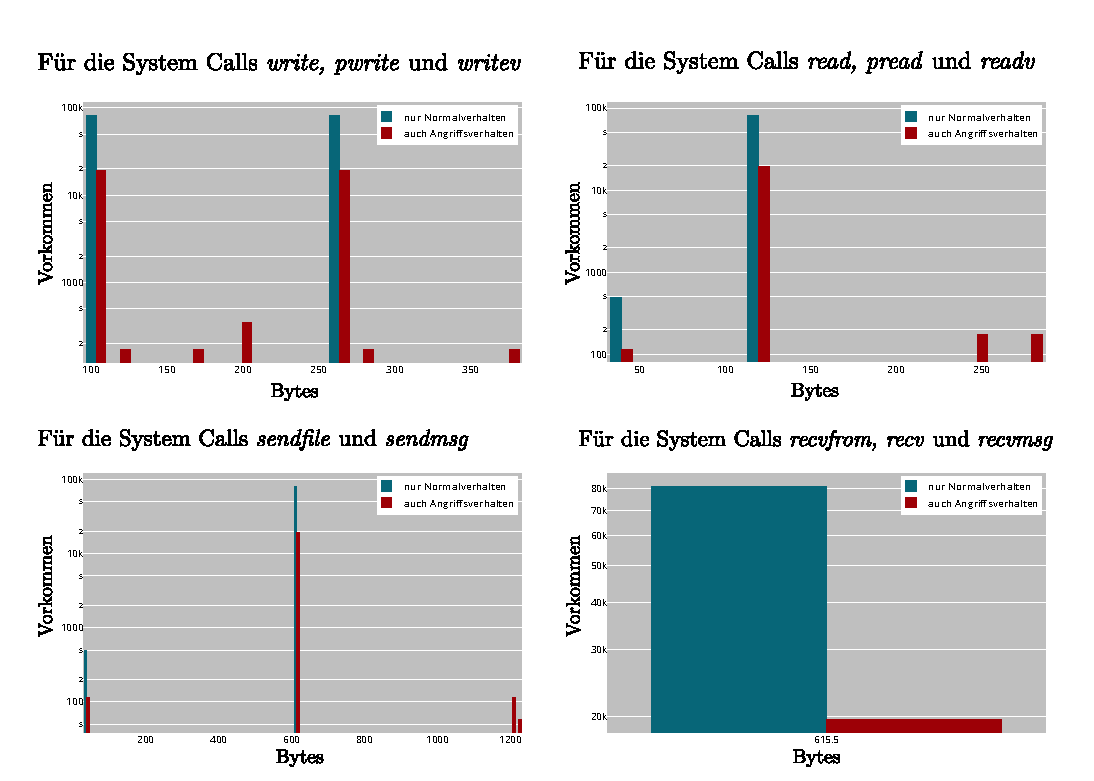
\includegraphics[width=\textwidth]{images/return_2017_plot.pdf}
                        \caption[Histogramm der geschriebenen und gelesenen Bytewerte]{Histogramm der gelesenen/erhaltenen Bytes für die Testdaten des \ac{LID-DS}~\cite{LID-DS} $CVE-2017-7529$ Szenarios.
                        Dargestellt wird dabei immer der Anteil einer Rückgabewertgröße in Byte an allen Rückgabewertgrößen der besagten System Calls.
                        Links oben für die von den System Calls \textit{write, pwrite} und \textit{writev} geschriebenen Bytes.
                        Rechts oben für die von \textit{read, pread} und \textit{readv} gelesenen Bytes.
                        Links unten für die von \textit{sendfile} und \textit{sendmsg} über Sockets gesendete Bytes.
                        Rechts unten für die von \textit{recvfrom, recv} und \textit{recvmsg} über Sockets erhaltenen Bytes.
                        Blau: Nur Normalverhalten, Rot: Normalverhalten und Angriffsverhalten}
                        \label{fig:return_values}
                    \end{figure}

        \subsection{Darstellung eines System Call Streams}\label{sec:streamdarstellung}
            Nachdem die Kodierung eines System Calls und zwei weiterer Parameter neben dem Namen selbst besprochen wurde, soll in diesem Abschnitt die Abarbeitung mehrerer System Calls für den verarbeitenden Algorithmus behandelt werden.
            Dabei werden die Abfolge der System Calls des Datensatzes als ein kontinuierlicher Stream betrachtet.
            Dies ermöglicht den Einsatz der entwickelten Vorgehensweise in der Praxis auch im Live-Betrieb, sofern die Verarbeitung entsprechend schnell stattfindet.
            Für viele Algorithmen wie zum Beispiel auch neuronale Netze ist es sinnvoll und teilweise unausweichlich, eine feste Eingangsgröße festzulegen.
            Um dies für einen Stream zu ermöglichen, werden in der \ac{NLP} schon seit langer Zeit N-Gramme verwendet~\cite{NGRAMSUEN1979}.
            Auch in der auf System Call basierten Anomalieerkennung kommen N-Gramme zum Einsatz~\cite{STIDE_Alternatives, SYSCALL_GRAPHS, IDSTHREADGRIMMER2021}.
            Ein N-Gramm ist eine zusammenhängende Folge von $n$ Elementen aus einer gegebenen Eingabe.
            Diese werden, wie in der linken Grafik in \autoref{fig:ngram_thread} beispielhaft dargestellt, aufgebaut.

            Dabei wird ein Buffer der Länge $n$ erzeugt, welcher das erste n-gram liefert, sofern sich $n$ Elemente in dem Buffer befinden.
            Kommt ein neues Element in den Buffer, fällt das älteste heraus.

            Zu beachten ist dabei, dass die Abfolge der System Calls mehrere logische Abfolgen zusammenführt.
            Denn moderne Computer Systeme verarbeiten mehrere Threads parallel.~\cite{SYSCALL_SILBERSCHATZ}
            Die System Calls aller Threads werden dann, je nach dem wie sie vom Betriebssystemskernel verarbeitet werden, an die Sequenz angefügt.
            
            \paragraph{Thread Awareness}
                Grimmer et al.~\cite{IDSTHREADGRIMMER2021} beschreiben in ihrer Arbeit wie sie die Thread Information der System Calls verwenden, um die verwundenen Sequenzen zu entwirren.
                Dabei wird für jeden Thread ein eigener Buffer erzeugt. 
                Die Ausgabe dieser Buffer wird in der rechten Grafik in \autoref{fig:ngram_thread} veranschaulicht. 
            Also nur System Calls aus demselben Thread bilden ein n-gram, weshalb sie von \textit{Thread aware} N-Grammen\marginpar{zu dt.\ Thread bewusst} sprechen.
                Grimmer et al.\ konnten zeigen, dass dies speziell auch für diesen Datensatz eine Verbesserung der Ergebnisse erzielt.
                Darüber hinaus zeigen sie, dass bei der Verwendung von \textit{Thread aware} N-Grammen im Vergleich zu n-grammen ohne Berücksichtigung von Threads in keinem Szenario eine Verschlechterung der Ergebnisse auftritt.

                \begin{figure}
                    %thread ngram image
                    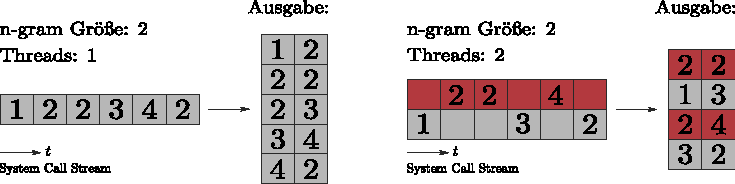
\includegraphics[width=\textwidth]{images/ngram.pdf}
                    \caption[Erstellung N-Gramme]{Erstellung der N-Gramme mit $n=2$ aus einem Datenstream von System Calls.
                        Links ohne und rechts mit der Beachtung der Threadinformation.
                        Die dabei entstehenden N-Gramme dienen als Eingabe für den bewertenden Algorithmus.
                        Die Reihenfolge der entstehenden N-Gramme als Eingaben ist dabei von oben nach unten.
                    }\label{fig:ngram_thread}
                \end{figure}

            \paragraph{Thread Change Flag}
                Sie verwenden in der Auswertung aber ausschließlich Algorithmen, welche kontextfrei arbeiten.
                Dies bedeutet, dass zuvor gesehene N-Gramme keinen Einfluss auf das aktuelle haben.
                Wie in~\autoref{sec:LSTM} beschrieben wird, ist das bei \ac{LSTM} Netzwerken nicht der Fall.
                Es gilt also den benötigten Kontext in die von Grimmer et al.\ beschriebene Methodik zu integrieren.

                Eine Möglichkeit bestünde darin, die ThreadID zu kodieren und die Information, aus welchem Thread das n-gram stammt, mitzugeben.
                Doch das Kodieren der tatsächlichen Thread ID ist sehr unpraktisch, da Thread IDs wiederverwendet werden können.
                Stattdessen wird in dieser Arbeit ein n-gram mit der Informatione über einen Kontextwechsel angereichert. 
                Dieser Kontextwechsel soll dann über die \ac{TCF} an das \ac{LSTM} übergeben werden.
                Initial wird, weil kein Kontextwechsel stattfindet, für die \ac{TCF} eine $0$ angegeben.
                Kommt das aktuelle n-gram aus demselben Thread wie das n-gram zuvor, ist die \ac{TCF} ebenfalls $0$.
                Ist das aktuelle n-gram allerdings aus einem anderen Thread, wird ein Kontextwechsel durch das Setzen der \ac{TCF} auf $1$ angezeigt.
                Visualisiert wird dies in \autoref{fig:ngram_tcf}.

                \begin{figure}[ht]
                    %thread ngram image
                    \centering
                    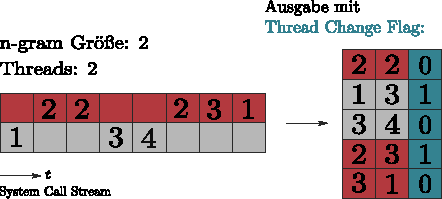
\includegraphics[width=0.6\textwidth]{images/tcf.pdf}
                    \caption[Erstellung Thread Aware N-Gramme]{Analog zu \autoref{fig:ngram_thread} werden N-Gramme erzeugt.
                             Diese werden nun mit der \ac{TCF} angereichert.
                             Initial ist die \ac{TCF} $0$.
                             Ist das zuvor ausgegeben n-gram aus demselben Thread, ist die \ac{TCF} ebenfalls $0$.
                             Findet ein Wechsel des Threads statt, wird dieser Kontextwechsel durch das Setzen der \ac{TCF} auf $1$ signalisiert.}\label{fig:ngram_tcf}
                \end{figure}

                Die Vorstellung dabei ist, dass eine \ac{TCF}$= 1$ dem \ac{LSTM} die Information gibt, dass die zuvor gesehenen N-Gramme nur eine untergeordnete Rolle für den Kontext spielen, da diese aus einem anderen Thread stammen.
                Falls dies der Fall ist, kann ein häufiger Kontextwechsel dafür sorgen, dass der Vorteil der \ac{LSTM}s abgeschwächt wird, da immer dafür gesorgt wird, dass potentiell wenige Informationen im Kontext enthalten sind.
                In \autoref{tab:tcf} wird dargestellt, wie oft so ein Kontextwechsel stattfindet.
                Dabei ist zu erkennen, dass in den Szenarien aus dem \ac{LID-DS} bei einer Länge von $n=6$ nur bis zu $13.8\%$ der N-Gramme eine $\ac{TCF}=1$ haben.
                Die zuvor geschilderte Gefahr scheint also für die gegebenen Szenarien keine Rolle zu spielen, ist aber für andere Einsatzbereiche mit nicht kontextfreien verarbeitenden Algorithmen zu beachten.

                \begin{table}[ht]
                    \small
                    \centering
                    \begin{tabular}{lrrr}
                        \hline
                        \rowcolor{GruvGray!36}
                        \multicolumn{4}{c}{Thread Change Flag}\\
                        \toprule
                        Szenario & \#\ac{TCF}$=1$ & \#\ac{TCF}$=0$ & \makecell{Anteil \ac{TCF}$=1$ \\an allen N-Grammen \\ in \%}\\
                        \midrule
                        \rowcolor{GruvGray!16}
                        $Bruteforce\_CWE\_307$ & $2,534,165$ & $20,383,314$ & $11.1$ \\
                        $CVE-2012-2122$ & $1,206,151$ & $10,365,309$ & $10.4$ \\
                        \rowcolor{GruvGray!16}
                        $CVE-2014-0160$ & $1,120,786$ & $7,026,864$ & $13.8$ \\
                        $CVE-2017-7529$ & $1,130,717$ & $10,721,010$ & $9.5$ \\
                        \rowcolor{GruvGray!16}
                        $CVE-2018-3760$ & $1,453,876$ & $38,255,576$ & $3.7$ \\
                        $CVE-2019-5418$ & $3,131,792$ & $74,159,462$ & $4.1$ \\
                        \rowcolor{GruvGray!16}
                        $PHP\_CWE-434$ & $10,891,051$ & $112,549,739$ & $8.8$ \\
                        $EPS\_CEW-434$ & $12,657,844$ & $374,439,042$ & $3.3$ \\
                        \rowcolor{GruvGray!16}
                        $ZipSlip$ & $80,126,899$ & $444,510,136$ & $15.3$ \\
                        \hline
                    \end{tabular}
                    \caption[Häufigkeit eines Kontextwechsels]{Vorkommen von eines Kontextwechsels angezeigt durch die \ac{TCF}.
                    Bei einer n-gram Länge von $6$.}
                    \label{tab:tcf}
                \end{table}

    \section{Aufbau des \NoCaseChange{\acp{LSTM}}}\label{sec:aufbau_lstm}
    \sectionmark{Aufbau des LSTMs}
        \begin{figure}[ht]
            \centering
            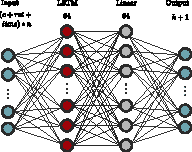
\includegraphics[width=0.7\textwidth]{images/lstm.pdf}
            \caption[Aufbau des \ac{LSTM}]{Aufbau des \ac{LSTM} mit $64$ Neuronen für die \ac{LSTM}- und Linear-Layer.
                Die Input Layer besitzt $(e + ret + time) * n$ Neuronen, mit $e$ für die Größe des \ac{W2V}-Embeddings,
                $ret=1$ falls Rückgabewerte verwendet werden und $time=1$ falls die Zeitabstände verwendet werden.
                Ansonsten sind $ret=0$ und $time=0$.
                Und die Output Layer hat $k+1$ Ausgangsneuronen, dabei ist $k$ die Anzahl an System Calls aus dem Trainingsdatensatz.
                Eins wird addiert für unbekannte System Calls.}
                \label{fig:lstm}
        \end{figure}

        Die Architektur wird ebenfalls in \autoref{fig:lstm} dargestellt und besteht aus der Eingabe-Layer, der \ac{LSTM}-Layer, einer \textit{fully-connected} Linear-Layer und der Output-Layer.
        Wie dargestellt, wird für die Initialisierung der Implementierung des \acp{LSTM} die Anzahl an Input und Output Neuronen benötigt.
        Für die Eingangsgröße gilt:
        \begin{equation}
            input\_dim = (e + ret + time) \cdot n + \ac{TCF}
        \end{equation}
        Mit $e$ für die gewählte Größe des \ac{W2V}-Embeddings.
        Falls der zuvor beschriebene Zusatzparameter für die Rückgabewerte verwendet wird gilt $ret=1$ ansonsten $ret=0$.
        Gleiches gilt für den Extraparameter, welcher die Zeitabstände kodiert und Kontextwechsel angebende \ac{TCF}.
        Für die Ausgangsgröße gilt:
        \begin{equation}
            output\_dim = k + 1
        \end{equation}
        Dabei ist $k$ die Anzahl an System Calls aus dem Trainingsdatensatz.
        Für unbekannte System Calls, welche in den Trainingsdaten nicht vorkamen, wird zusätzlich noch eins addiert.
        Nötig ist diese Variabilität, da für die Initialisierung des \acp{LSTM} die Anzahl der verschiedenen System Calls im Trainingsdatensatz für die Ausgangsgröße, sowie die Eingangsgröße des System Calls eine entscheidende Rolle spielt.

        Festgelegt werden hingegen Größen für die \textit{Hidden Layer} Dimension, \textit{Batch Size}, den \textit{Optimizer}, die \textit{Loss}-Funktion und die Lernrate.
        Die Dimension der \ac{LSTM}-Layer wird auf $64$ gesetzt, die \textit{Batch Size} auf $1024$.
        Es wird der für \acp{LSTM} gängige \textit{Adam Optimizer} gewählt.
        Da es sich um eine Klassifikation mit $k+1$ Klassen handelt, wird die \textit{Cross-Entropy} Loss-Funktion des PyTorch Frameworks genutzt.
        Die Lernrate wird auf $0.001$ festgelegt.
        Details zu der Parameterwahl wird in \autoref{sec:parameterwahl} erläutert.

        Entgegen der typischen Implementierungen von \acp{LSTM} wird der \textit{Hidden State} nach einem Batch gespeichert und dem nächsten Batch  übergeben. 
        Der Hauptgrund dafür ist die Länge der System Call Streams.
        Diese können länger als ein Batch sein.
        Standardmäßig werden die Hidden States nicht übergeben, weswegen die Kontextinformation zwischen den Batches verloren geht.
        Diese Idee ist allerdings ausgelegt für einen kontinuierlichen Stream an System Calls, der Datensatz besteht aber aus vielen Dateien.
        Deswegen wird der \textit{Hidden State} zum Ende einer Aufnahme zurückgesetzt.

        Ausgaben des \acp{LSTM} sind durch die Verwendung der PyTorch CrossEntropy Loss-Funktion sogenannte \textit{Logits}.
        Auf diese kann mithilfe der \textit{Softmax}-Funktion eine Liste an Wahrscheinlichkeiten für jeden System Call sowie den Platzhalter erstellt werden.

    \section{Algorithmus}\label{sec:Algorithmus}
        Im vorigen Kapitel wurden alle verwendeten Vorverarbeitungsschritte vorgestellt.
        In den kommenden Abschnitten werden diese Schritte zu einem Ablauf zusammengeführt.
        Zunächst soll in \autoref{sec:Allgemein} ein allgemeiner Überblick gegeben werden.
        Anschließend wird in \autoref{sec:Training} behandelt, was das \ac{LSTM} Netzwerk lernt.
        Schließlich erklären \autoref{sec:Anomalieerkennung} und \autoref{sec:Schwellung}, wie aus dem Gelernten die Klassifizierung in normales oder Angriffsverhalten erfolgt.

        \subsection{Allgemein}\label{sec:Allgemein}
            Wie bereits in \autoref{sec:related_nlp} beschrieben, werden verschiedene Verfahren der \ac{NLP} auch in der anomaliebasierten \ac{HIDS} eingesetzt.
            Neben den bereits beschriebenen \ac{W2V} Verfahren, kommen auch die in der \ac{NLP} verbreiteten \ac{LSTM} Netzwerke zum Einsatz.
            Mit dem \ac{LSTM} soll in der Trainingsphase ein Sprachmodell der System Calls erstellt werden.
            Dieses Sprachmodell soll mit einer gegebenen Sequenz $s = (sc_{x_1},\dots,sc_{x_n})$ den folgenden System Call $sc_{x_{n+1}}$ vorhersagen. 
            Dabei bestehen die Trainingsdaten nur aus Normalverhalten, enthalten also keine Angriffe.
            Anhand dieses gelernten Modells soll dann in der Testphase eine Vorhersage über den nächsten System Call gemacht werden.
            Diese Vorhersage besteht aus den Wahrscheinlichkeiten für alle aus dem Training gesehenen System Calls, plus einem Platzhalter für noch unbekannte System Calls.
            Die Wahrscheinlichkeit des tatsächlich auftretenden System Calls von eins abgezogen, stellt dann den Anomaliescore dar.
            Ob dieser Anomaliescore zu einem Alarm führt oder nicht, hängt von einem zuvor bestimmten Schwellwert ab.
            Dieser wird bestimmt, indem nach dem Training die Anomaliescores für einen Ausschnitt des Datensatzes bestimmt werden.
            In diesem Ausschnitt, auch Validierungsdaten genannt, darf wie in den Trainingsdaten kein Angriffsverhalten enthalten sein.
            Eine Garantie, die in der echten Welt nie komplett gegeben werden kann.
            In den Validierungsdaten soll folglich kein Alarm ausgelöst werden, weshalb der höchste Anomaliescore der Validierungsdaten als Schwellwert der Anomalieerkennung verwendet wird.
            Dies ist eine Annäherung an einen optimalen Schwellwert.

            Die System Calls werden wie zuvor beschrieben durch das \ac{W2V} Verfahren in einen Vektor umgewandelt und durch die zwei zuvor beschriebenen Verfahren, die Normalisierung der Zeitabstände und der Rückgabewerte bestimmter System Calls, angereichert.
            Der Stream der System Calls wird dann mit Betrachtung der Threads in N-Gramme zusammengetragen.
            Zusätzlich wird zu jedem n-gram die Information über einen Kontextwechsel durch die \ac{TCF} angegeben.
            % Im Folgenden wird der Trainingsablauf detaillierter bestimmt.

        \subsection{Training}\label{sec:Training}
            \begin{figure}
                \centering
                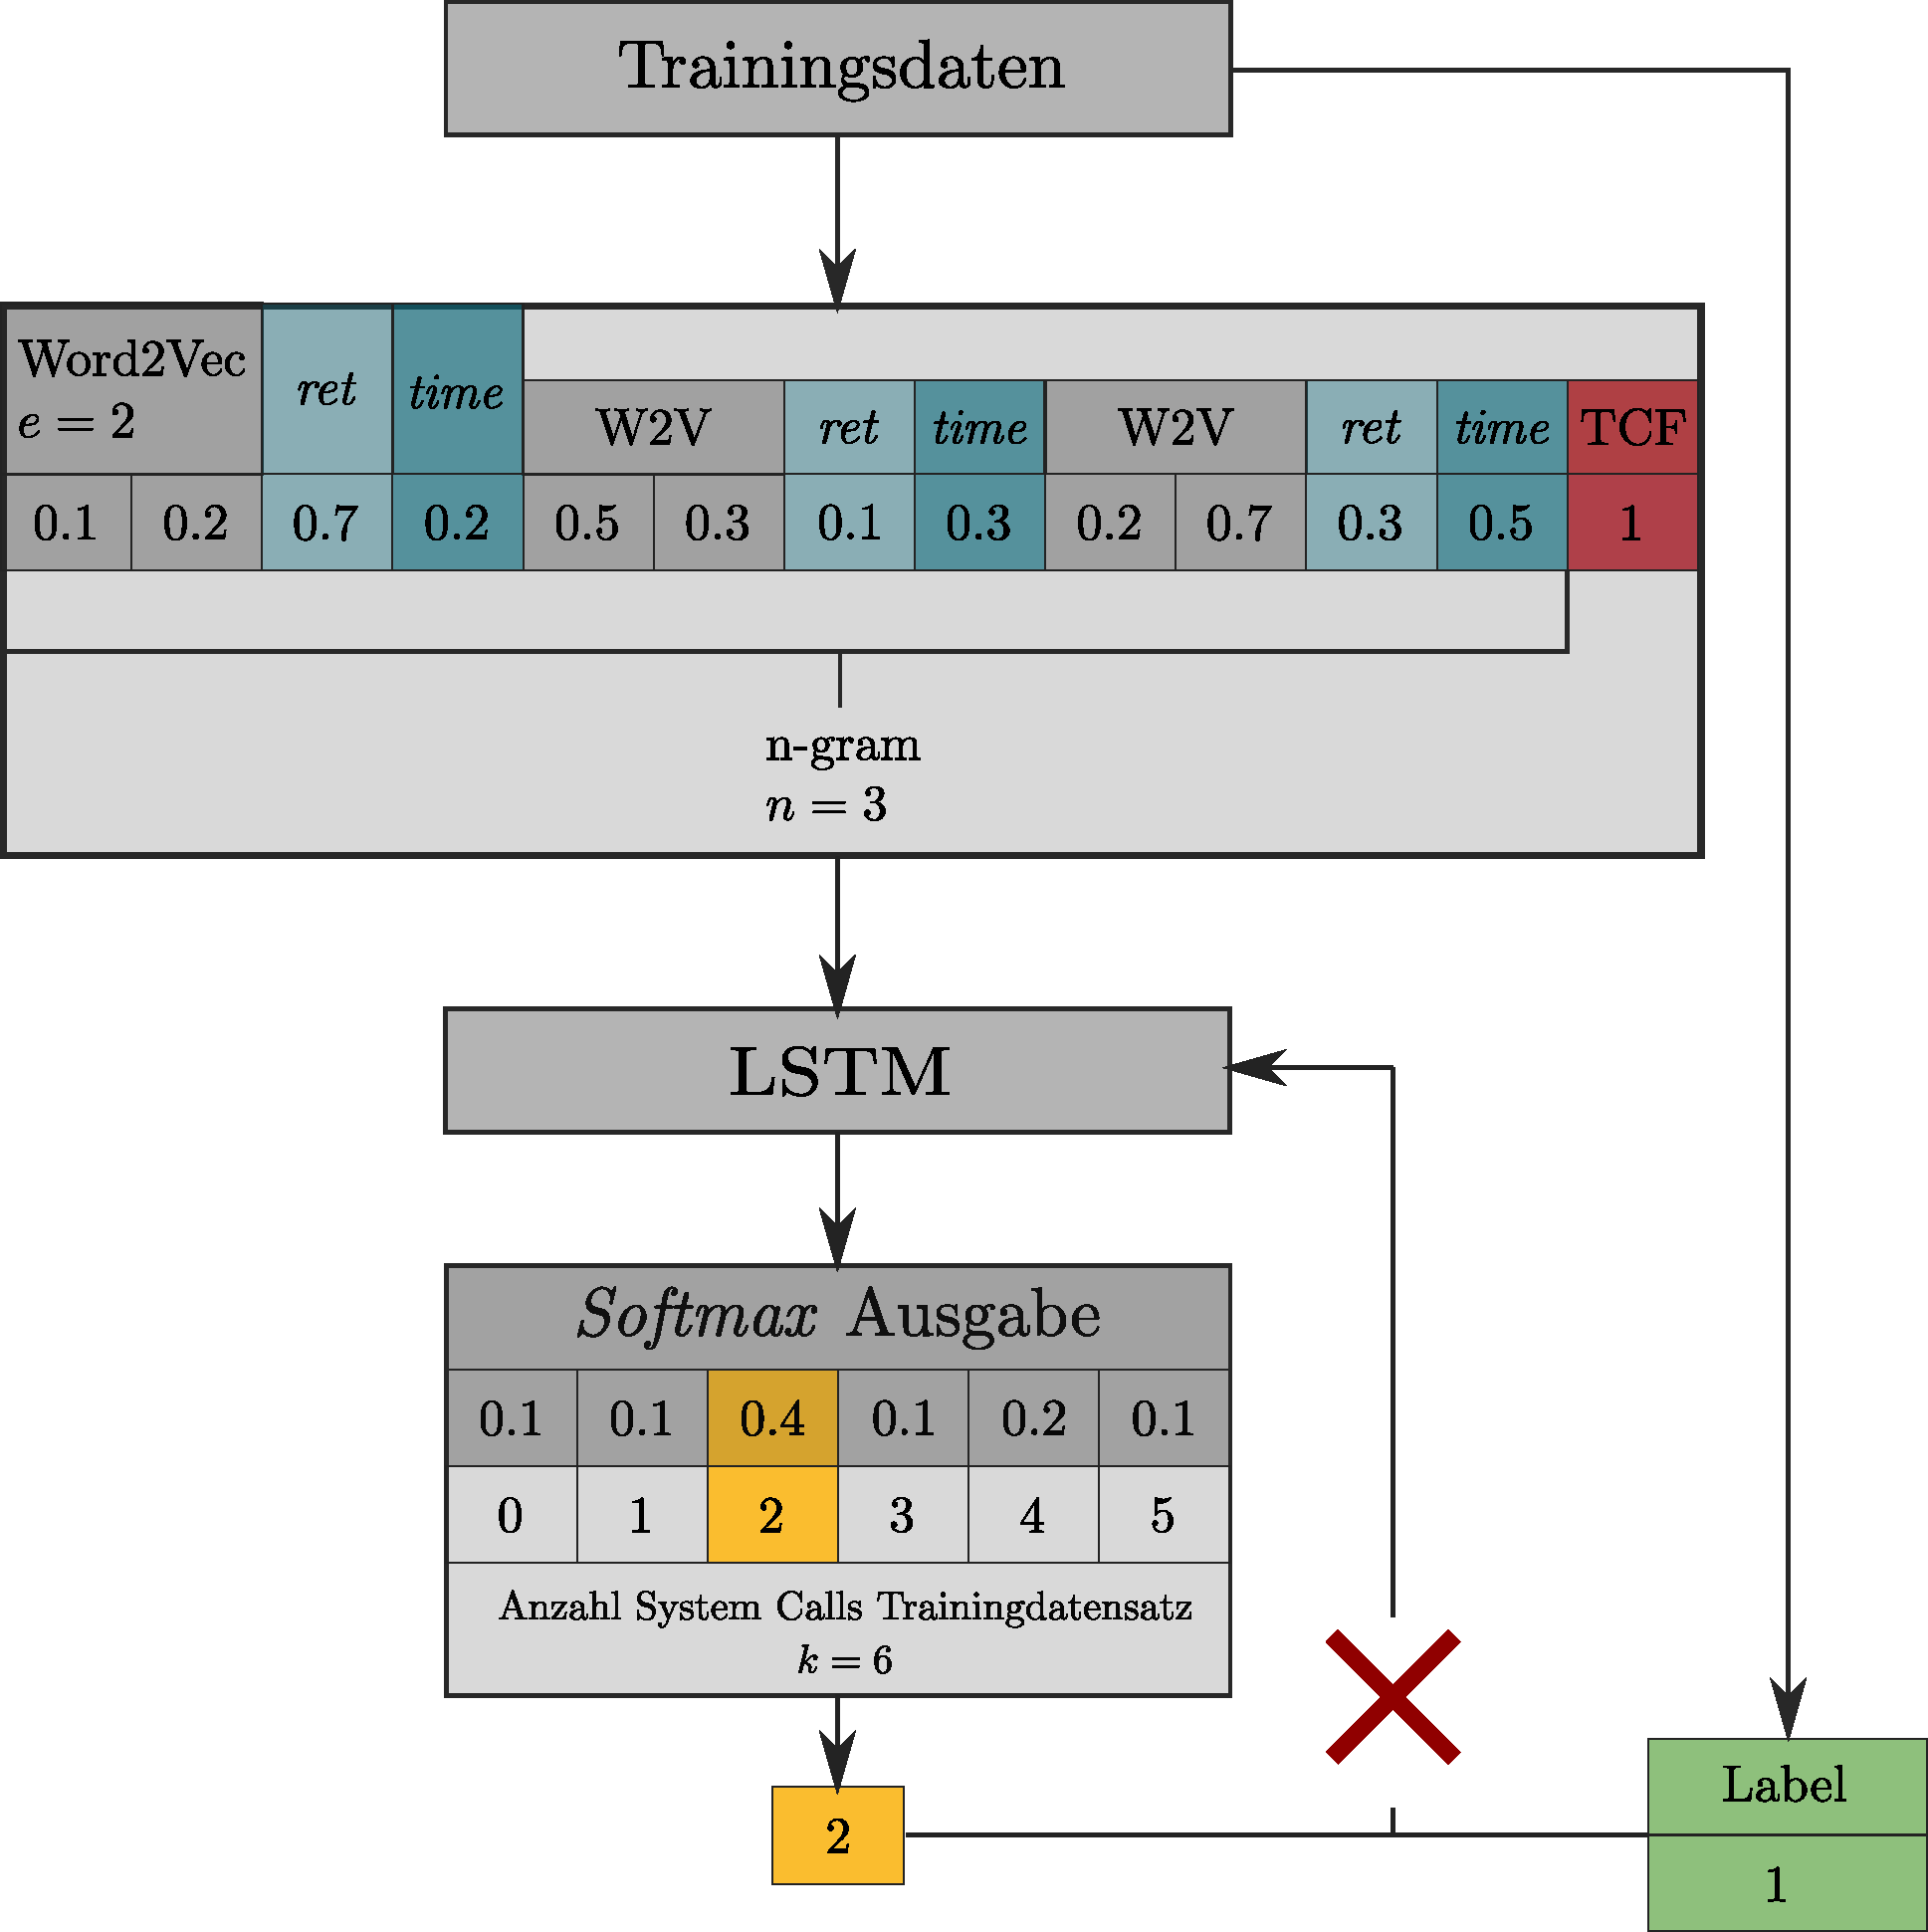
\includegraphics[width=0.75\textwidth]{images/Process_overview.pdf}
                \caption[Algorithmus - Ablauf Trainingsphase]{Ablauf der Trainingsphase mit Beispieldaten.
                        Aus Trainingsdaten wird ein n-gram aus \ac{W2V}, Rückgabewert (\textit{ret}) und Zeitabstand (\textit{time}) erstellt.
                        Diese beiden Extraparameter sind bläulich hervorgehoben.
                        Zusätzlich wird die \ac{TCF} an das n-gram gefügt.
                        Der Index des höchsten Wertes (gelb) aus der Ausgabe des \ac{LSTM} wird mit dem eigentlichen Label (grün) verglichen.
                        Aufgrund dieser Information werden die Gewichte im \ac{LSTM} angepasst}\label{fig:training}
            \end{figure}
            % Für das Training des \ac{LSTM} Netzwerkes werden nur Normaldaten aus dem Trainingsdatensatz verwendet.
            Pro Szenario werden $200$ Aufnahmen ohne Angriffsverhalten, der insgesamt ca.\ $1100$ Aufnahmen, für das Training ausgewählt.
            Die Grund\-idee besteht wie zuvor beschrieben darin, mit einer gegebenen Sequenz $s = (sc_{x_1},\dots,sc_{x_n})$ den folgenden System Call $sc_{x_{n+1}}$ vorherzusagen. 
            Da der nächste System Call aus dem Datensatz stets bekannt ist, kann als Feedback für das Netzwerk die Information genommen werden, ob $sc_{x_{n+1}}$ korrekt vorhergesagt wurde, also dem Label entspricht.
            Das \ac{LSTM} gibt wie in \autoref{fig:training} dargestellt diese Information an das \ac{LSTM} zurück.

            Seien die System Calls aus den Trainingsdaten aus der Menge $SC = \{sc_1,sc_2,\dots,sc_k\}$.
            Womit $k$ die Anzahl der in den Trainingsdaten vorkommenden System Call Namen angibt.
            Die Trainingsdaten werden durchlaufen und N-Gramme $ngram_i$ erstellt.
            Der auf das $ngram_i$ folgenden System Call dient als Label $l_i$.
            Nach dieser Idee ist das erste n-gram $ngram_0$ mit Label $l_0$.
            Dabei werden die System Call Namen für die Label durch Integerwerte ersetzt. 
            Das \ac{LSTM} Netzwerk bekommt $ngram_0$ und gibt einen Vektor der Länge $k+1$ zurück.
            Dieser Vektor gibt für jeden der $k$ möglichen System Calls aus den Trainingsdaten eine Auftrittswahrscheinlichkeit an.
            Zusätzlich wird $1$ addiert, da in den Testdaten unbekannte System Calls auftreten können.
            Diese bekommen den \ac{W2V}-Vektor $(0)^e$, wobei $e$ die Länge des \ac{W2V}-Vektoren ist oder für das Label einen Integerwert von $0$. 
            Die Ausgabe des \acp{LSTM} sind \textit{PyTorch Logits}, diese werden mithilfe der \textit{Softmax}-Funktion in die gewünschten Wahrscheinlichkeiten umgewandelt.
            Der Index der Liste der so berechneten Wahrscheinlichkeiten wird mit dem aus den Trainingsdaten gezogenen Label verglichen.
            Dieser Vergleich dient dann als Feedback für das \ac{LSTM}.
            Mit den gegebenen Trainingsdaten kann nun das \ac{LSTM} mittels des \textit{back-propagation through time}  trainiert werden.

        \subsection{Anomalieerkennung}\label{sec:Anomalieerkennung}
            \begin{figure}[ht]
                \centering
                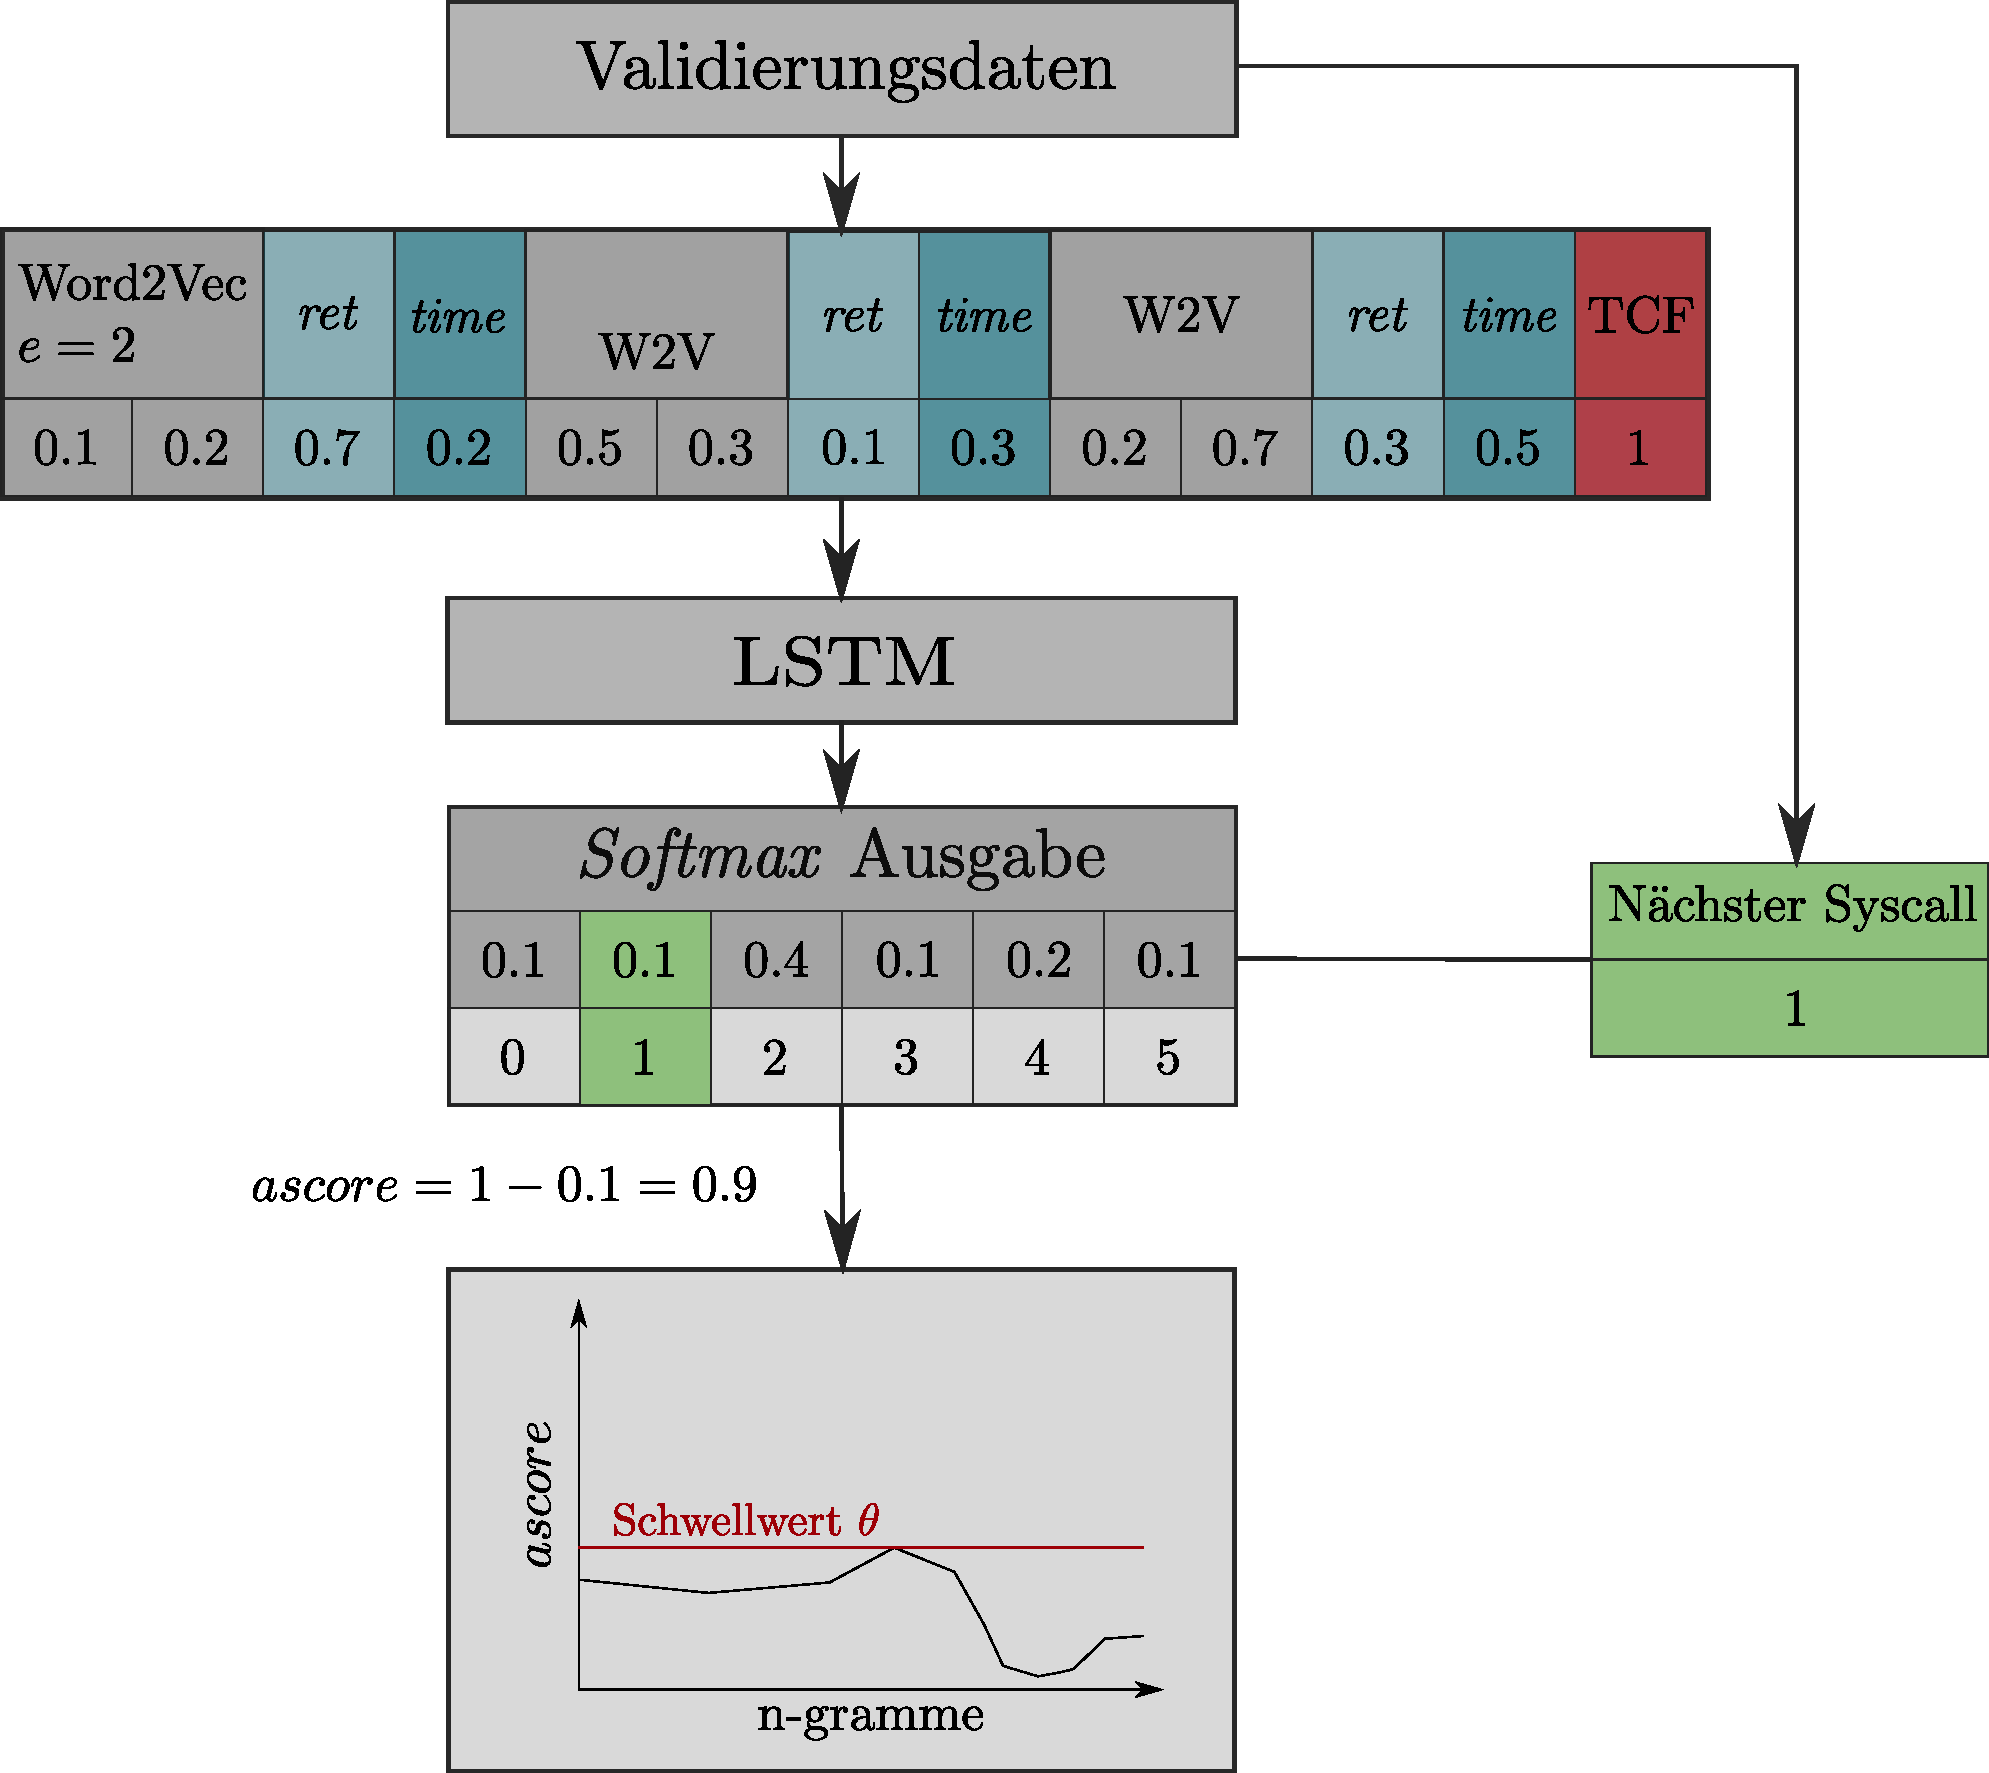
\includegraphics[width=0.8\textwidth]{images/Validation_overview.pdf}
                \caption[Algorithmus - Ablauf Validierungsphase]{Ähnlich zu \autoref{fig:training} wird hier der Validierungsablauf beschrieben.
                         Dabei wird wie zuvor ein Datenauszug dargestellt sowie die Auftrittswahrscheinlichkeiten für den folgenden System Call.
                         In der Test-, wie in der Validierungsphase dient die Wahrscheinlichkeit des Integerwerts des tatsächlich als nächstes auftretende System Call als Berechnungsgrundlage für den Anomaliescore.
                        Wie unten in der Abbildung dargestellt, wird das Maximum der $ascore$s der gesamten Validierungsdaten als Schwellwert festgelegt.}
                \label{fig:validierung}
            \end{figure}
            Es kann also bei Auftreten des System Calls $sc_i$ überprüft werden mit welcher Wahrscheinlichkeit $p_i$ dieser vorhergesagt wurde.
            Der eigentliche Anomalie-Score $ascore$ für $sc_i$ wird dann folgenderweise berechnet:
            \begin{equation}
                ascore = 1 - p_i
            \end{equation}
            Übertrifft dieser Wert einen zuvor bestimmten Schwellwert $\theta$, so wird $sc_i$ als Anomalie und damit als Angriff gewertet.

            \paragraph{Schwellwertbestimmung}\label{sec:Schwellung}
                Für die Berechnung des Schwellwertes $\theta$ wird für alle System Calls der Validierungsdaten $ascore$ berechnet.
                Die Validierungsdaten bestehen aus $50$ Aufnahmen und enthalten ebenfalls wie die Trainingsdaten nur das Normalverhalten.
                Da in den Validierungsdaten kein Angriffsverhalten integriert ist, darf keiner der $ascore$s einen Alarm auslösen.
                Weshalb der höchste Wert der $ascore$s der Validierungsdaten als Schwellwert $\theta$ genutzt wird.
                Der Ablauf der Schwellwertfindung wird zusätzlich in \autoref{fig:validierung} dargestellt.
                Dabei ist ähnlich zu \autoref{fig:training} dargestellt, wie ein System Call n-gram kodiert wird und als Eingabe in das \ac{LSTM} dient.
                Zusätzlich wird die Berechnung des $ascores$ dargestellt, indem das Label als Index für die Softmax  Ausgabe des \acp{LSTM} dient.
                Das Maximum der $ascores$ wird, wie beschrieben, dann als Schwellwert $\theta$ genutzt.

        \subsection{Parameterwahl}\label{sec:parameterwahl}
            Das Aufsetzen des beschriebenen Algorithmus bedarf der Festlegung einiger Parameter.
            Dazu gehören allgemeine Parameter für neuronale Netze, aber auch spezifischere Parameter wie die Länge der N-Gramme.
            Da nicht alle Parameter experimentell untersucht werden können, werden sie im Folgenden in festgelegte und zu ermittelnde Parameter unterteilt.
            \paragraph{Festgelegte Parameter}
                Entscheidende Parameter der \acp{LSTM} sind die Anzahl der Neuronen pro Layer sowie die Anzahl der \ac{LSTM}-Layer in dem Netzwerk.
                Da sich bei ersten Tests schnell die Problematik aufgetan hat, dass die Berechnungen sehr großer Szenarien zu nicht tragbaren Laufzeiten führt, muss dies bei der Findung vieler Parameter bedacht werden.
                Deshalb wird in dieser Arbeit nur eine \ac{LSTM}-Layer verwendet, auch wenn in manchen Anwendungen der \ac{NLP} mehrere Layer zu einer verbesserten \textit{Accuracy} führen.\cite{LSTMHYPERAUFA2020}
                Die Anzahl der Neuronen dieser Layer wird wie bereits in \autoref{sec:aufbau_lstm} beschrieben auf $64$ festgelegt.
                Die Lernrate wurde anhand der Ergebnisse mehreren Tests auf wenigen Szenarien auf $0.001$ festgelegt.
                Außerdem wird der für \acp{LSTM} häufig eingesetzte Adam-Optimizer verwendet.
                Diese Einstellungen wurden auch in der Arbeit von Dymshits et al.~\cite{LSTMDYMSHITS2017} eingesetzt.
                Als Loss Funktion wird für das $k+1$ Klassen Klassifizierungsproblem die \textit{Cross-Entropy} gewählt.
                Wie auch in \autoref{fig:learning_rate} erkennbar ist, stagniert der Fehler bei verschiedenen Szenarien nach nur wenigen Epochen, weshalb für die Epochenanzahl ein Maximum von $20$ festgelegt wird.
                Der Einfluss der Batch size auf die Ergebnisqualität wird unter anderem in~\cite{LSTMBENCHBREUEL2015} als gering eingestuft und wird auf $1024$ festgelegt.
                 
                
                \begin{figure}
                    \centering
                    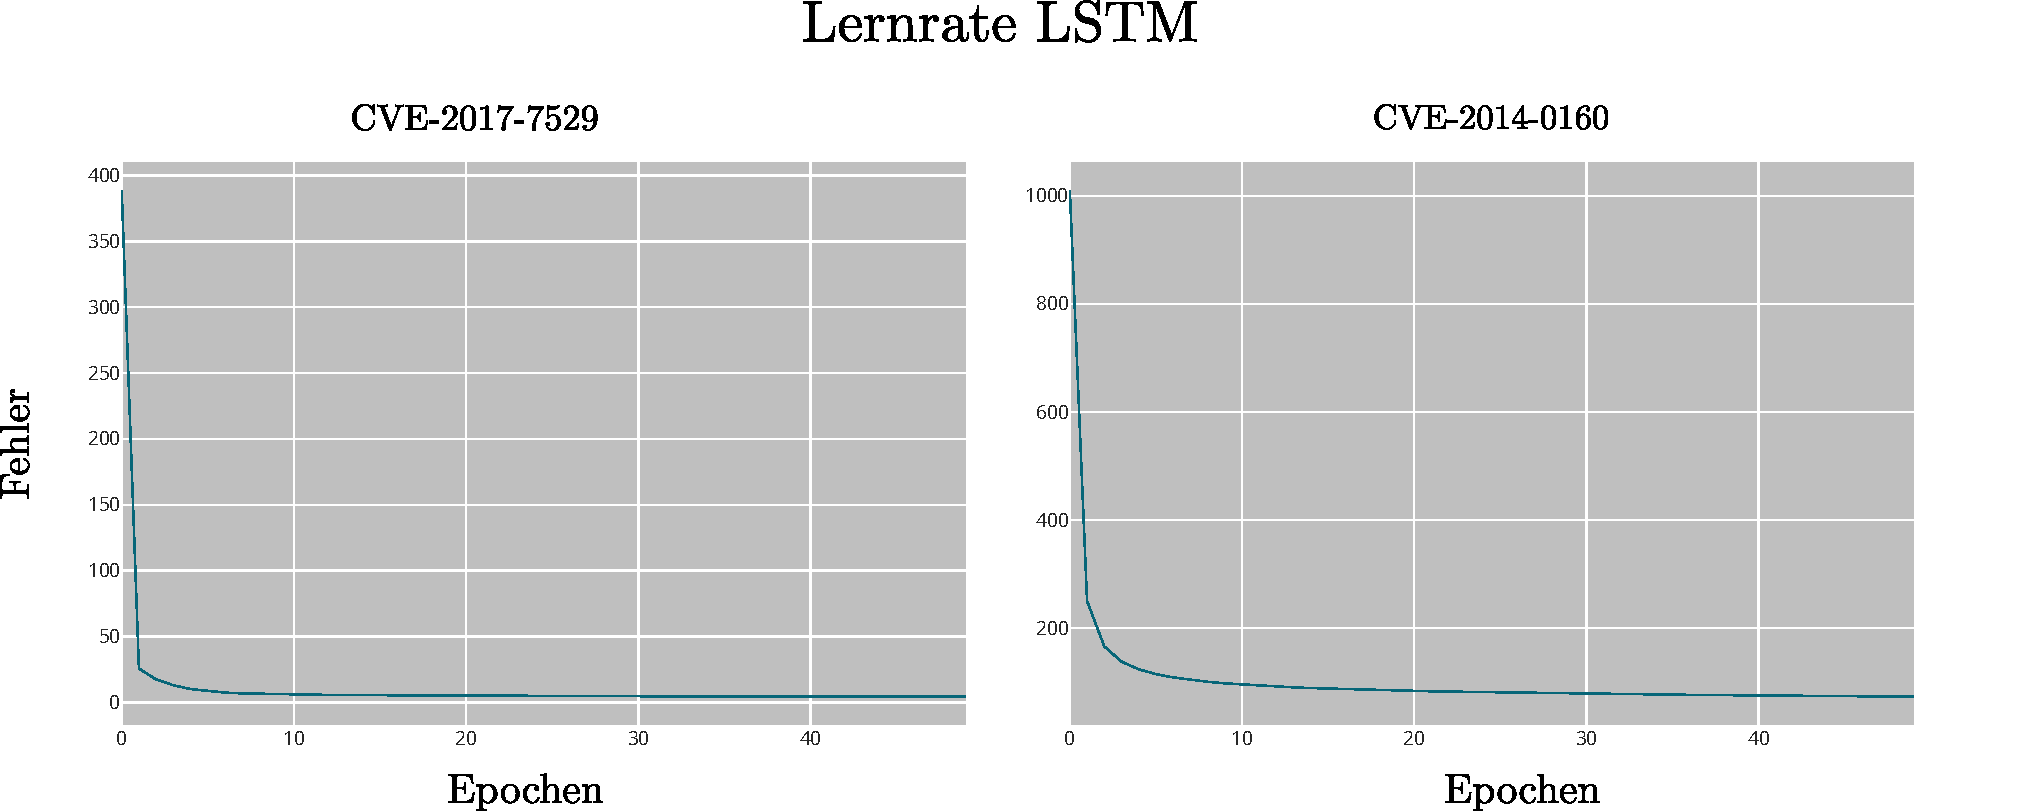
\includegraphics[width=\textwidth]{images/learning_rate.pdf}
                    \caption[Parameterwahl - Fehler während des Trainings]{Darstellung des Fehlers während des Trainingsvorgangs für zwei Szenarien.
                             Zum einen ist ein Lernfortschritt zu erkennen und zum anderen tritt dieser bereits nach wenigen Epochen ein.}\label{fig:learning_rate}
                \end{figure}

                Da das Berechnen des \ac{W2V} im Vergleich zum Training und Testen des \acp{LSTM} nur einen geringen Zeitaufwand benötigt, wird eine Epochenanzahl von $500$ festgelegt. 
                Es werden aufgrund der Ergebnisse von Grimmer et al.~\cite{IDSTHREADGRIMMER2021} nach verschiedenen Tests mit alten Konfigurationen nur N-Gramme mit Betrachtung der Thread Information aufgebaut.

            \paragraph{Zu ermittelnde Parameter}
            Ziel ist es eine Konfiguration der Parameter zu finden, mit der alle Szenarien aus dem \ac{LID-DS} mit hoher \ac{DR} und niedriger \ac{FP}-Rate ausgewertet werden können.
            Dafür gilt es speziell verschiedene \textbf{n-gram} Größen in Kombination mit verschiedenen Größen für das \textbf{\ac{W2V}-Embedding} zu finden.
            Für die n-gram Größen wurden $[2,6,10]$ und für das \ac{W2V}-Embedding $[4,6,8,10]$ zur Auswahl gestellt.
            Zusätzlich soll untersucht werden, ob sich durch die Hinzunahme weiterer System Call Parametern neue erfolgreiche Konfigurationen ergeben.
            Speziell wird getestet, ob sich \textbf{\ac{TCF}}, \textbf{Rückgabewerte}, \textbf{zeitliche Abstände} oder jegliche \textbf{Kombinationen} dieser positiv auf die Ergebnisse auswirken.
                
\iffalse
    \section{Strukturierung der Experimente}\label{sec:StrukExp}
        Um aussagekräftige Experimente zu entwickeln müssen zuerst 
        überlegungen zur praktischen umsetzung gemacht werden
        dabei wird in ersten Tests klar, dass zeit hierbei eine große rolle spielen wird

        erste Tests also ausgelegt um Faktoren zu ermitteln, welche die auswertungen stark verlangsamen
        und diese ausschließen.

        \subsection{Faktor Zeit}
            zeit/dr als groesse und farbe von scatter plot
            batch size test und train x/y achse

            eingrenzen von moeglichen konfigurationen

            Berechnungszeiten aus verschiedenen Perspektiven relevant:
            soll live system werden
            begrenzte rechenleistung und viele Tests zur auswertung von parametern architektur etc
            erster test zur abschätzung diverser zeitl.\ faktoren:

            Faktoren:
            \begin{itemize}
                \item Architektur
                \item Verarbeitung Stream

                     ngram größe
                \item embedding
            \end{itemize}
            ngram größe, architektur und verwendung w2v statt ohe
            Grobe Abschätzung der Zeit, da Berechnungen auf Clustern ausgeführt werden von Auslastung beeinflusst werden.
            Klare Erkenntnisse:
            Single Small 50 neuronen eine schicht:
            Single Big 250 neuronen eine schicht
            multi 50 neuronrn 3 schichten
            erste Abschätzung von Nutzen von Thread 
            einführen von stateful sowie Batch Normalization
        \subsection{Optimale Parameter}
            \paragraph{Architektur}
                versch architekturen:
                Single Small 50 neuronen eine schicht
                Single Big 250 neuronen eine schicht
                multi small 20 neuronen 3 schichten
                multi big 50 neuronrn 3 schichten
                deep erste 50 sonst 20 6 schichten

                singlesmall 43\% von Deep
                insgesamt am schnellsten single small
                wie zu erwarten,  deep am langsamsten

                teste eine schicht viele neuronen 
                eine schicht wenige neuronen
                mehrere schichten mehrere neuronen / mit dropout dazwischen
                viele schichten wenige neuronen /mit dropout dazwischen

                auf Grund des zeitlichen Faktors fallen Deep und multibig weg
                Also zu testen:
                Single Small
                Single 
                Multi Small
                Multi 

            \paragraph{Hyperparameter}
                aktivierungs funktion
                -> dense layer with softmax or tanh
                batch size
                learning rate
                optimizer

            \paragraph{Ngram Größe}
                ngram größer -> langsamer

            \paragraph{Threadinfo}
                Hypothese:
                Threadinfos bringen was

                Einbinden von thread information auf verschiedenen wegen:
                Thread aware ngrams (tan)
                Thread aware ngrams for w2v (tanw2v)
                Thread change flag (tcf)

                varianten:
                tan
                tanw2v
                tcf
                tan tcf
                tan tanw2v
                tcf tanw2v
                tan tanw2v tcf

                ---> welcher dieser varianten am besten?

            \paragraph{Parameter}
                args
                time

                \ac{LSTM} ohne Threadinfos mit OHE
                LSTM mit W2V ohne Threadinfos (ngram)
                LSTM mit W2V mit Threadinfos (ngram)
                LSTM mit W2V threadaware mit Threadinfos (ngram)
                LSTM mit W2V threadaware mit Threadinfos (ngram) und threadchangeflag
                LSTM mit W2Vthreadaware mit Threadinfos (ngram) und threadchangeflag, spezialtraining
                --> LSTM final

                Manche angriffe verändern Sequenz von syscalls nicht
                Hypothese:
                verwende Parameter um erg zu verb

                LSTM final + strlen
                LSTM final + time delta
                LSTM final + strlen + time delta

                \fi

\section{Metriken}\label{sec:Metriken}

    Typische Metriken für die Auswertung von neuronalen Netzen und damit auch für \acp{LSTM}, welche auch in der Anomalieerkennung eingesetzt werden, umfassen die \textit{Precision}, \textit{Recall} und den \textit{F1-Score}.
    \begin{figure}
        \centering
        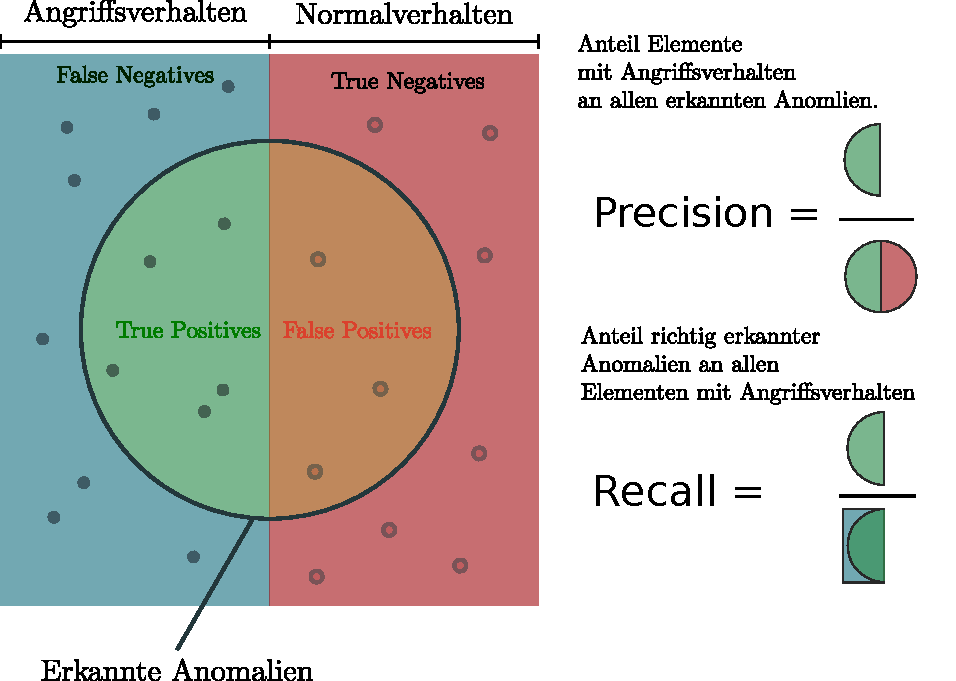
\includegraphics[width=0.75\textwidth]{images/Illustrationen/Precision.pdf}
        \caption[Darstellung Precision und Recall]{Visualisierung der Berechnung der häufig verwendeten Metriken der Precision und des Recalls, bezogen auf die Domäner der \textit{Intrusion Detection}.}\label{fig:metriken}
    \end{figure}
    Diese werden, wie in \autoref{fig:metriken} dargestellt, berechnet.
    Da der Datensatz aus System Calls besteht, bedeutet Recall in diesem Fall der Anteil an korrekt erkannten bösartigen System Calls an allen bösartigen System Calls.
    Wie in \autoref{sec:prob_LIDDS} beschrieben liefert der Datensatz allerdings nur den Angriffszeitpunkt und keine Label für jeden einzelnen System Call.
    Also muss jeder System Call nach dem Angriffszeitpunkt als bösartig eingestuft werden, obwohl neben dem Angriffsverhalten noch Normalverhalten stattfindet.
    Wird von einem optimalen Fall ausgegangen, dass alle dem Angriff zugehörigen System Calls einen Alarm auslösen, wird der Recall immer noch sehr niedrig sein und damit keinen realistischen Wert liefern.
    Somit ist auch der F1-Score wenig nützlich, da sich dieser aus Recall und Precision zusammensetzt.
    Es scheint deshalb sinnvoller andere Metriken zur Hand zu nehmen, um einheitliche und vom Datensatz unabhängige Messwerte bereitstellen zu können. 
    Da der \ac{LID-DS} aus vielen verschiedenen Aufnahmen besteht, kann die Berechnung der Precision und des Recalls auch auf Dateiebene stattfinden.
    Falls mehrere Angriffe in einer Datei vorkommen, wird die Berechnung jedoch umständlicher, dies ist im \ac{LID-DS} nicht der Fall.  
    Grundgedanke der Findung einer neuen Metrik muss dabei auch sein, einen klaren Praxisbezug zu finden. 
    Dort ist vor allem interessant, wieviele Angriffe erkannt werden und nicht wieviele System Calls der Angriffe als bösartig eingestuft werden.
    Zum anderen entscheidet die Anzahl, beziehungsweise die Häufigkeit von Fehlalarmen über die Nutzbarkeit der \acp{IDS}.
    Die \ac{DR} steht für den zuvor beschriebenen Recall auf Dateiebene, also der Anteil der erkannten Angriffe an allen vorkommenden Angriffen.
    Werden alle Aufnahmen mit Angriffsverhalten korrekt erkannt gilt: $\ac{DR}=1$.
    Dabei wird außer Acht gelassen, dass ein Alarm nach dem Angriffszeitpunkt wie in \autoref{sec:prob_LIDDS} beschrieben, theoretisch auch ein Fehlalarm sein kann.
    Nur ein Alarm vor dem Angriffszeitpunkt oder in einer Aufnahme ohne Angriffsverhalten wird als Fehlalarm beziehungsweise als \ac{FP} gewertet.
    Zusätzlich gelten alle System Calls solange zu einem Alarm, bis der $ascore$ wieder unter dem Schwellwert $\theta$ liegt.
    Ziel ist es also, eine hohe \ac{DR} und eine möglichst geringe \ac{FP}-Rate zu erreichen.
    Um einschätzen zu können welche Konfiguration am besten abgeschnitten hat, ergibt sich eine neue Schwierigkeit.
    Es ist schwierig zu beurteilen, welche Konfiguration am besten funktioniert, denn wenn alle System Calls aus dem Datensatz als Angriff erkannt werden, ist $\ac{DR}=1$.
    Eine hohe \ac{DR} alleine ist also wenig aussagekräftig.
    In der Auswertung muss deswegen eine Abwägung zwischen \ac{FP}-Rate und \ac{DR} stattfinden.
    %Eine Angriff gilt dann als erkannt, sofern ein Alarm nach dem Angriffszeitpunkt ausgelöst wird. 
    %Wie in \autoref{sec:LIDDS} beschrieben werden dabei potentiell Fehlalarme als korrekt eingestuft.
    % Das sind im Folgenden die \ac{DR} und die \ac{FP}-Rate
